\chapter{Desenvolvimento}

Este capítulo detalha os processos que ocoreram no desenvolvimento da pesquisa, mostrando os passos seguidos para alcançar os objetivos propostos. Além disso, são abordadas as dificuldades enfrentadas e as adptações e refinamentos realizados ao longo do percurso.

\section{Circuito}

\subsection{Emissor}

O circuito que permite ``transformar" os bits em luz é composto por um led de alto brilho, um transistor TIP 122, dois resistores e uma bateria.

O transistor é ligado como chave na SBC para permitir acionar cargas eletricas da qual a SBC não seria capaz, como o led de alto brilho consome uma corrente maior poderia queimar a SBC.

\begin{figure}[!htbp]
  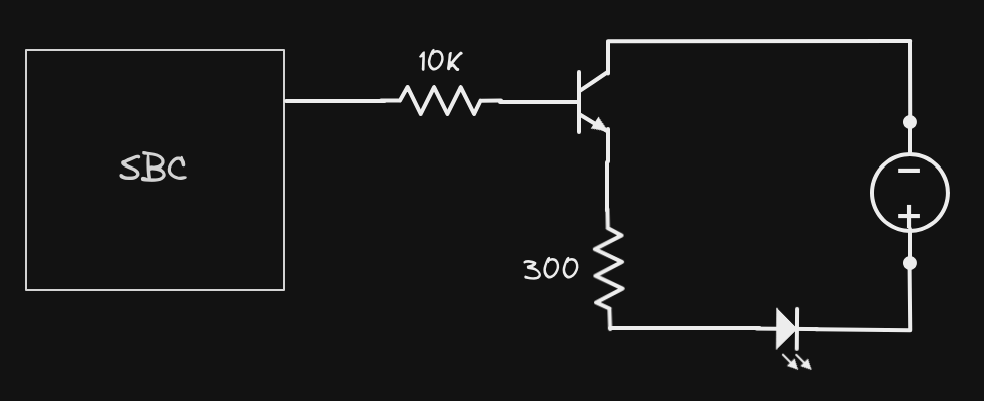
\includegraphics[width=0.5\textwidth]{images/esquema_circuito_emisor.png}
  \caption{Esquema do circuito emissor}
  \label{esquema-circuito-emissor}
\end{figure}

% TODO: Mudar para uma foto com iluminação
\begin{figure}[!htbp]
  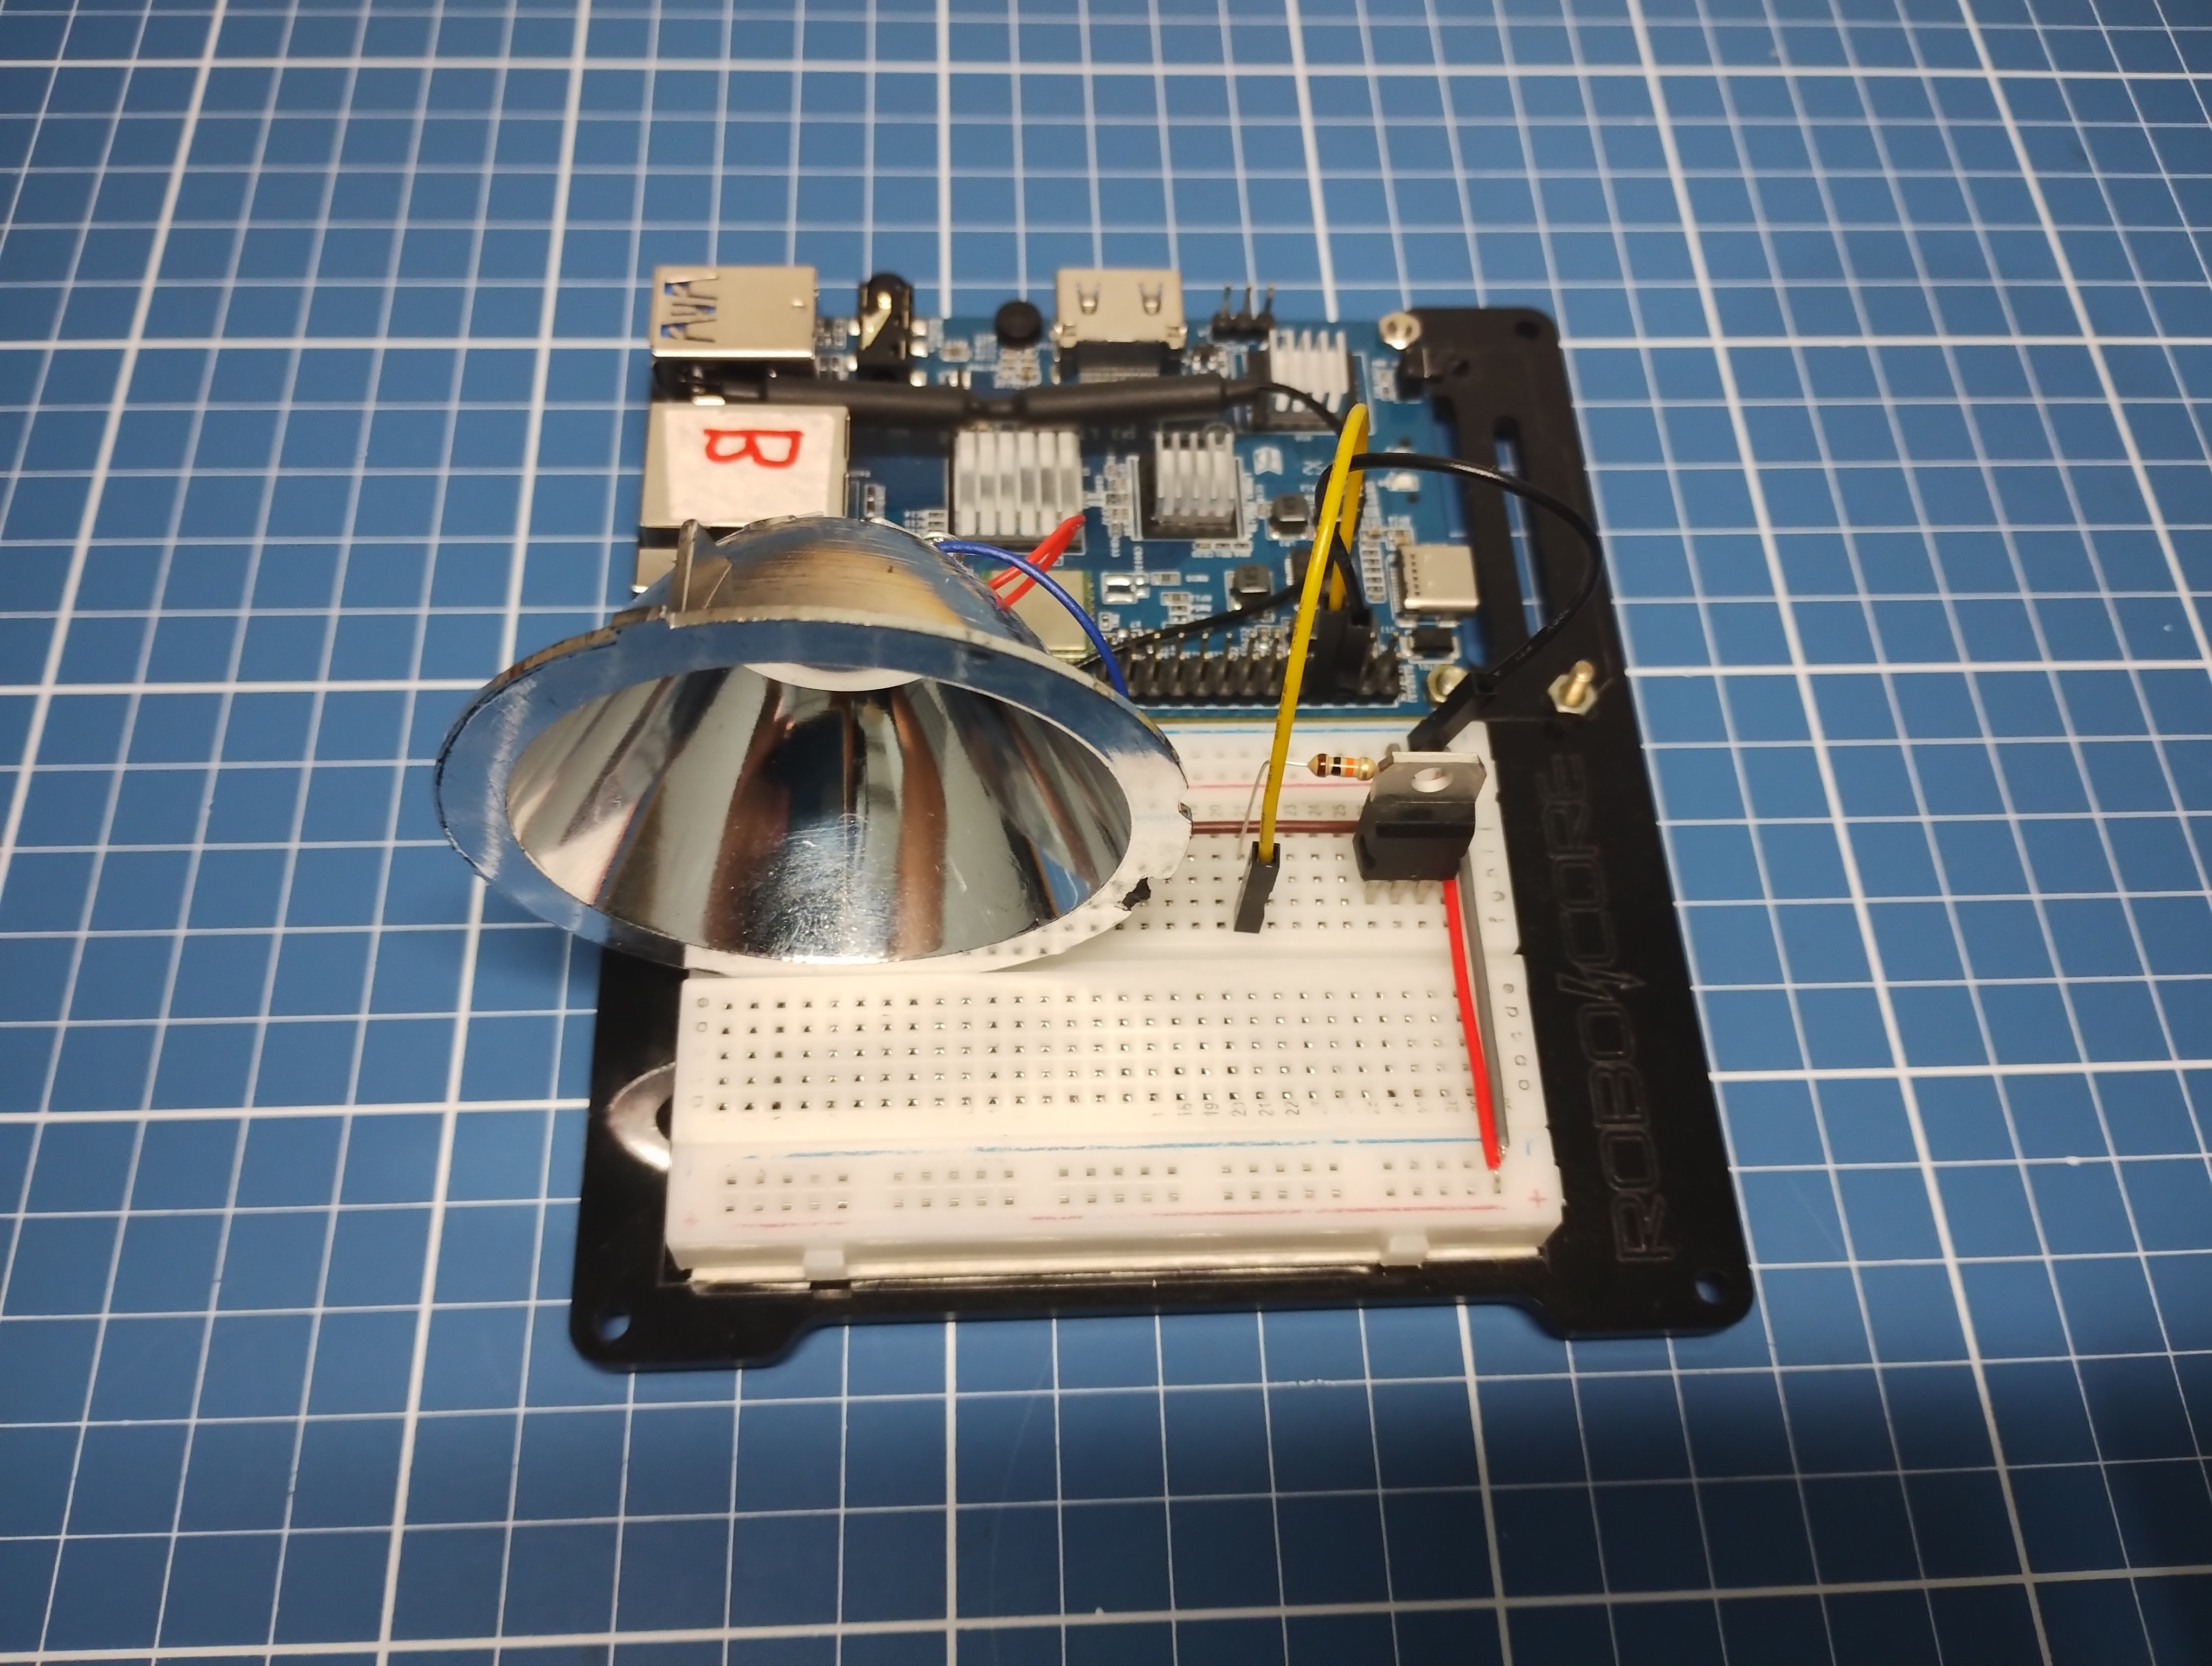
\includegraphics[width=0.4\textwidth]{images/foto_circuito_emisor.jpg}
  \caption{Esquema do circuito emissor}
  \label{foto-circuito-emissor}
\end{figure}


\subsection{Receptor}

O circuito para receber as informações do emissor é composto por um LDR (Light Dependent Resistor) e um potenciometro ligados em serie. Este circuito permite ler os \emph{bytes} indepentemente da intencidade da iluminação externa, ajustando a posição do potenciometro.

\begin{figure}[!htbp]
  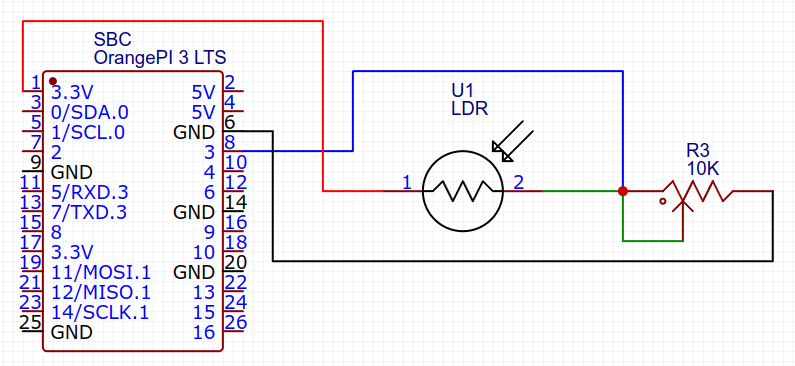
\includegraphics[width=0.5\textwidth]{images/esquema_circuito_receptor.png}
  \caption{Esquema do circuito receptor}
  \label{esquema-circuito-receptor}
\end{figure}


\begin{figure}[!htbp]
  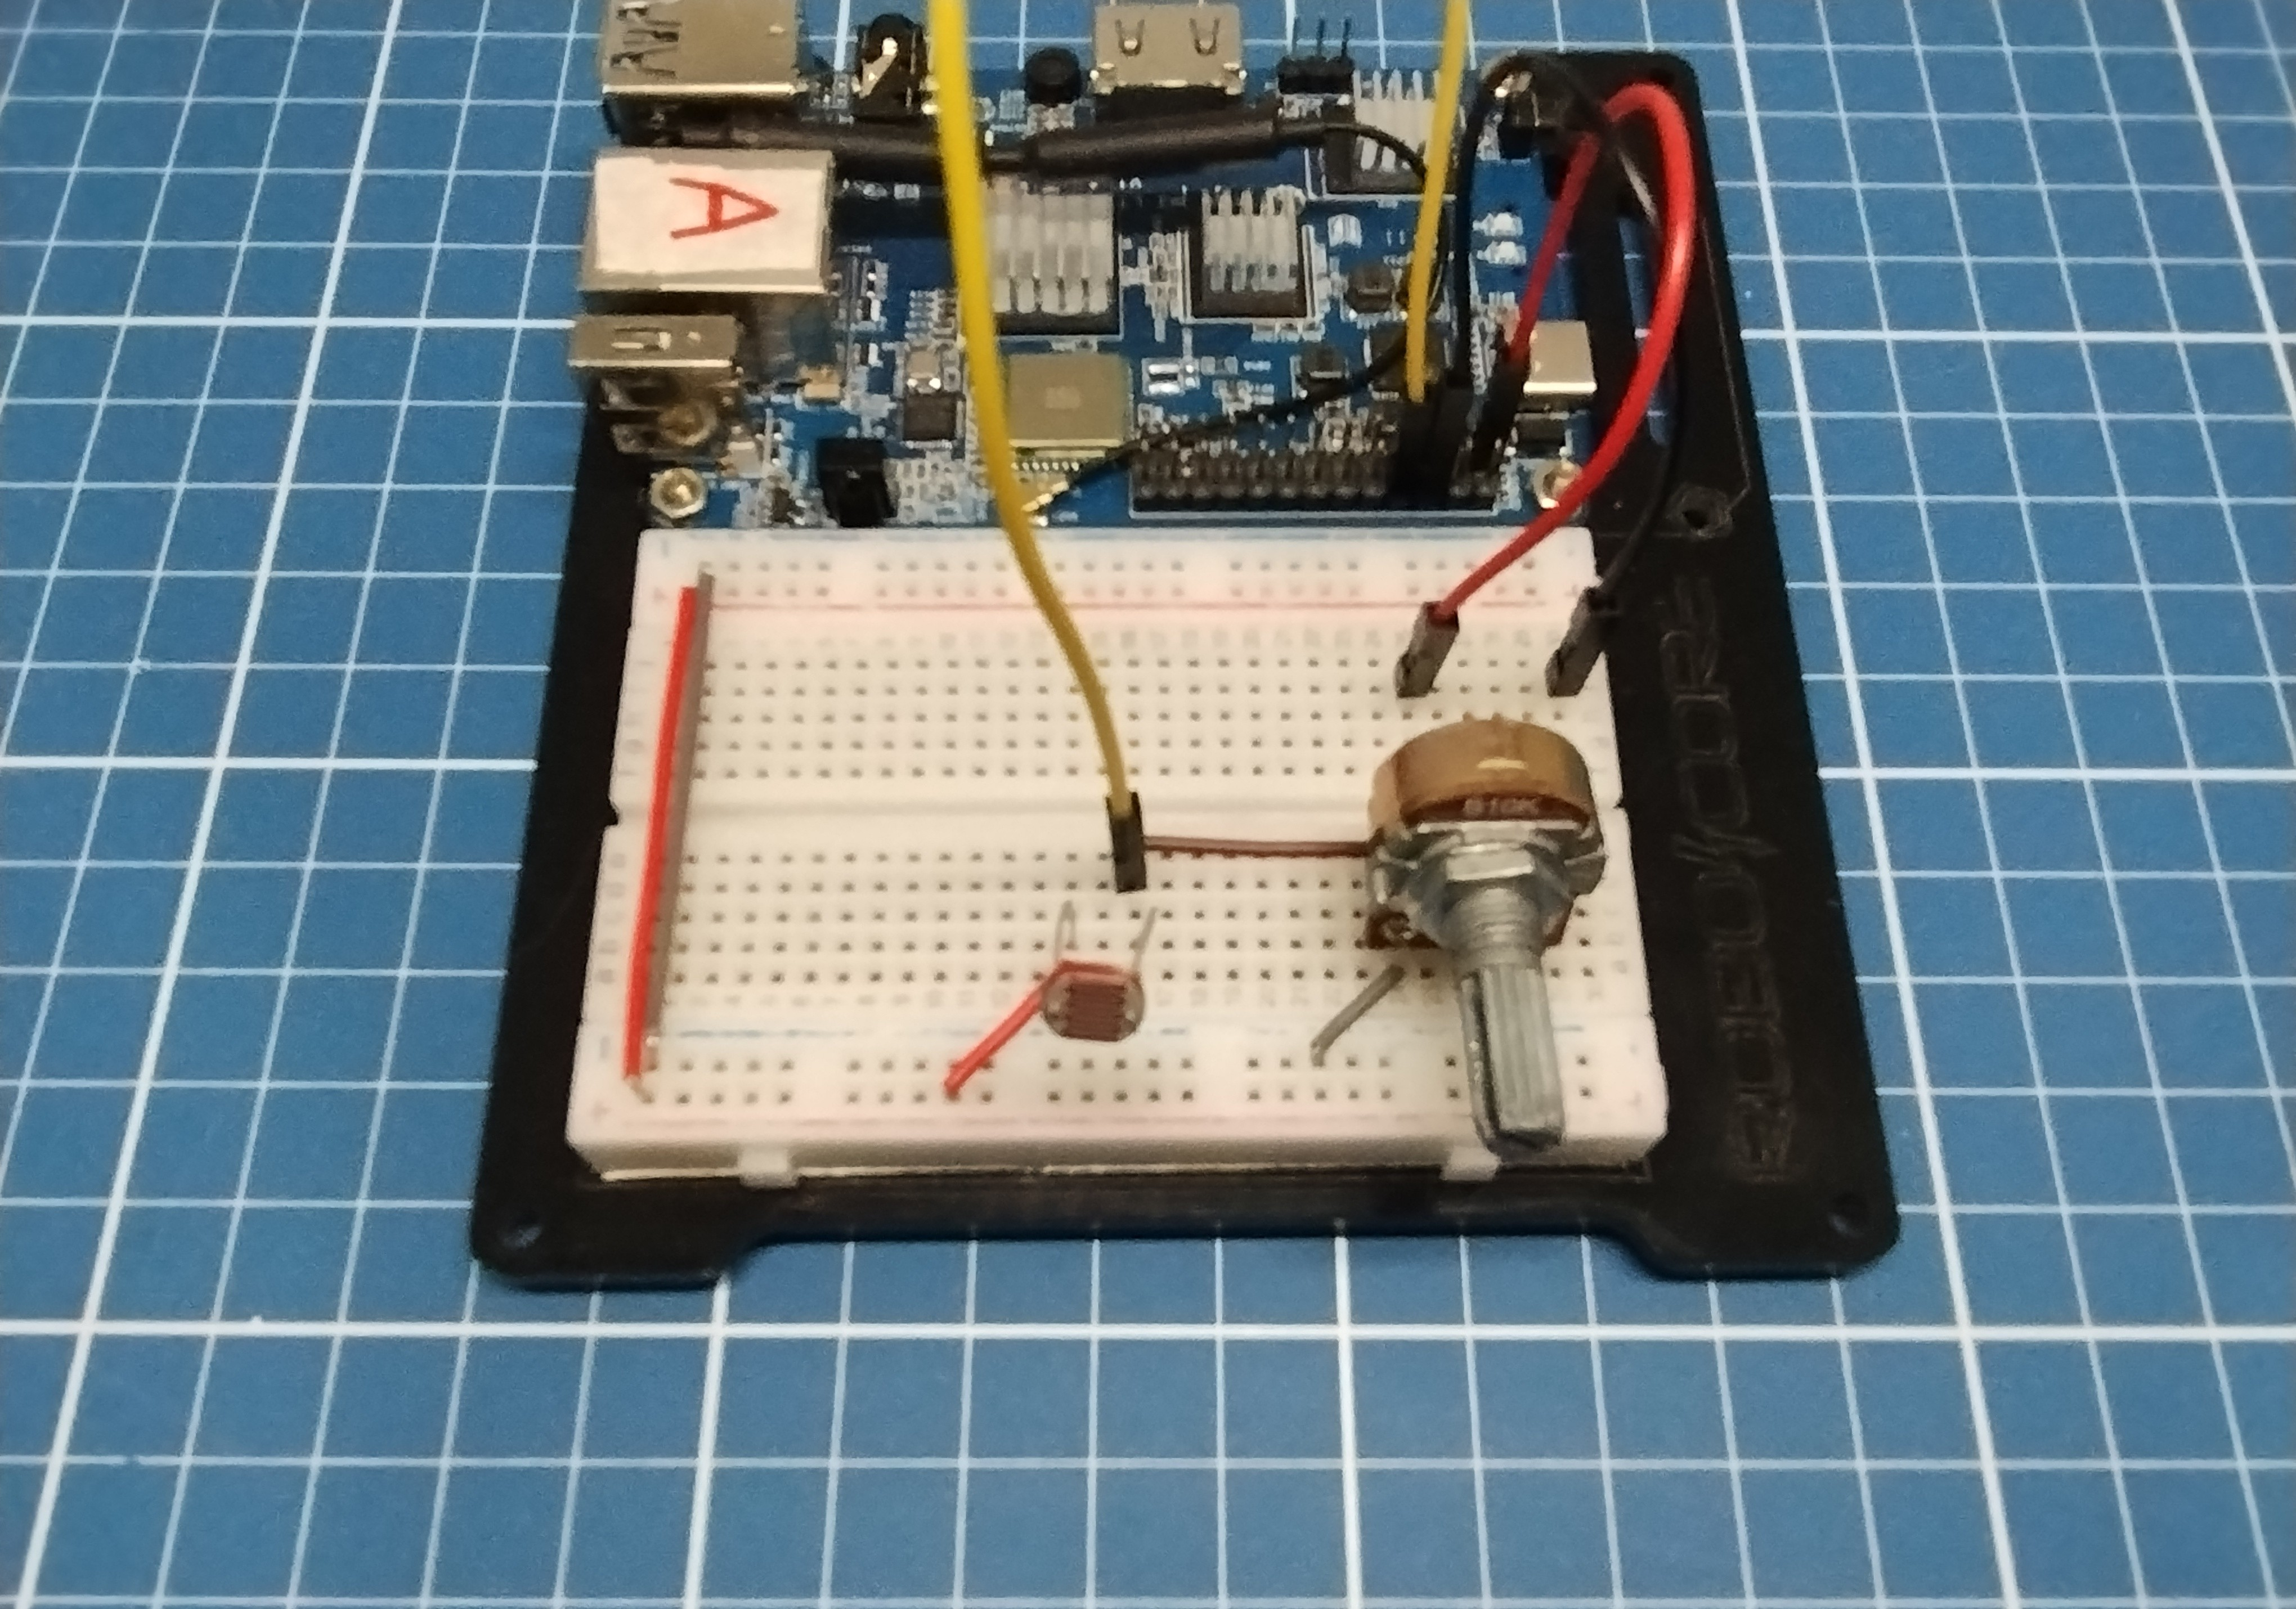
\includegraphics[width=0.4\textwidth]{images/foto_circuito_receptor.jpg}
  \caption{Esquema do circuito receptor}
  \label{foto-circuito-receptor}
\end{figure}

